\chapter{Implementación}
\section{Expresiones regulares}\label{imp:expresiones_regulares}
Se ha elegido esta forma de extraer los datos por ser una forma rápida y eficiente de extraer datos que comparten un patrón más o menos definido.
\subsection{Direcciones IP}
\subsubsection{IPv4}
Como se ha comentado en el apartado \ref{subsec:ipv4} una dirección IP en su versión 4 está definida por 4 números. Su valor va del 0 al 255 y están separados por un punto. 

Lo primero que se va a crear es una expresión regular que permita encontrar números del 0 al 255, tanto añadiendo ceros a la izquierda, como sin ellos. 

Esto se puede hacer de la siguiente forma: 
\begin{verbatim}
    25[0-5]|2[0-4][0-9]|[01]?[0-9][0-9]?
\end{verbatim}

Tal y como se puede ver, hay tres posibles alternativas: 
\begin{enumerate}
    \item \verb|25[0-5]|: Un número que empiece por 25 y termine con un número entre el 0 y el 5 ambos incluidos. Números incluidos den este rango [250-255].
    \item \verb|2[0-4][0-9]|: un número que empiece por dos, que esté sucedido de un número del 0 al 4 (El 5 se ha contemplado en la primera opción) y que finalmente esté sucedido de un tercer número del 0 al 9. Números incluidos den este rango [200-249].
    \item \verb|[01]?[0-9][0-9]?|: En este rango se contemplan todos los número del 0 al 199, ya sea empezando con ceros o sin ellos.  
\end{enumerate}
Esta expresión regular sólo detecta un número del 0 al 255, para detectar una dirección IPv4 completa sería necesario una expresión regular de la siguiente forma: 

\begin{lstlisting}[breaklines, caption={Expresión regular IPv4}, label={Regex:ipv4}, captionpos=b]
    (?:(?:25[0-5]|2[0-4][0-9]|[01]?[0-9][0-9]?)\.){3}(?:25[0-5]|2[0-4][0-9]|[01]?[0-9][0-9]?)
\end{lstlisting}

La expresión regular anterior se introduce en un grupo, al que se le agrega “\textbackslash.“ para detectar los puntos que separan los números. Con “\{3\}” se indica que va a haber exactamente 3 grupos de este tipo y finalmente se añade de nuevo la primera expresión regular para detectar el último número del 4 grupo, esta vez sin punto. 

\subsubsection{IPv6}
La expresión regular para detectar una dirección IP en versión 6 es mucho más compleja debido a la gran cantidad de posibles modificaciones que se pueden hacer.
Ya que una dirección IPv6 está formada por 8 números en hexadecimal cuyo valor puede ir del 0 al FFFF y se pueden escribir tanto en mayúsculas como en minúsculas. Estos números se pueden detectar mediante la siguiente expresión regular.

\begin{lstlisting}[breaklines, caption={Expresión regular para capturar un número exadecimal de 4 dígitos}, label={Regex:numero_hex}, captionpos=b]
                    [0-9a-fA-F]{1,4}
\end{lstlisting}

También es necesario tener en cuenta que los dos últimos números pueden ser sustituidos por una dirección IP en versión 4, para lo que se utilizará la expresión regular del apartado anterior (Código \ref{Regex:ipv4}), aunque se va a sustituir por “\verb!${ipv4}!” con el objetivo de facilitar la comprensión ya que, de otra manera, quedan expresiones tan largas que es complicado leerlas. 

La siguiente expresión regular puede capturar o bien dos números en hexadecimales separados por “:” o bien una dirección IPv4 y de aquí en adelante será sustituida por “\verb!${2groups_or_ipv4}!”:

\begin{lstlisting}[breaklines, caption={Expresión regular para capturar los dos últimos números o una dirección IP en versión 4}, label={Regex:2numeros_IPv4}, captionpos=b]
   (?:(?:[0-9a-fA-F]{1,4}:[0-9a-fA-F]{1,4})|${ipv4})
\end{lstlisting}

Por último, recordar que los números cuyo valor valga 0, se pueden contraer mediante “::”.

A continuación, se van a analizar nueve casos, puestos en orden de mayor a menor cantidad de posibles números contraídos, para así jugar con las posibles posiciones del valor “::”.

Esto se hace de esta manera para evitar que se capturen subpartes de la dirección y no la dirección completa.

\paragraph{Dirección completa}
En este caso se va a contemplar que la dirección esté completa y por tanto no haya ninguna contracción. 
En este caso la expresión es la siguiente: 

\begin{lstlisting}[breaklines, caption={Expresión regular para capturar dirección IPv6 completa}, label={Regex:ipv5_completa}, captionpos=b]
  (?:(?:(?:[0-9a-fA-F]{1,4}:){6})${2groups_or_ipv4})
 \end{lstlisting}

En ella se distinguen dos partes, la primera está compuesta simplemente por 6 números hexadecimales de 4 dígitos como ya se ha visto (Código \ref{Regex:numero_hex}), separados por “:” \verb!(?:(?:[0-9a-fA-F]{1,4}:){6})! y la segunda parte de la expresión también ha sido analizada (Código \ref{Regex:2numeros_IPv4}) y, o bien captura dos números hexadecimales separados por “:” o bien una dirección IPv4.

\paragraph{Contracción del primer número}

El siguiente caso detecta una dirección cuyo primer número está contraído. 

La expresión es muy similar a la anterior:

\begin{lstlisting}[breaklines, caption={Expresión regular para capturar dirección IPv6 con el primer número contraido}, label={Regex:ipv6_1}, captionpos=b]
   (?:(?:::(?:[0-9a-fA-F]{1,4}:){5})${2groups_or_ipv4})
\end{lstlisting}

Simplemente se añaden los “::” de la contracción y se reduce de 6 a 5 los posibles siguientes números hexadecimales.

\paragraph{Contracción del segundo número (Y tal vez del primero)}
En la contracción del segundo número hay que tener en cuenta que el primer número también puede estar contraido, por ejemplo la dirección:

\begin{verbatim}
    0000:0000:aaaa:bbbb:cccc:dddd:eeee:ffff
\end{verbatim}
Podría contraerse como:
\begin{verbatim}
    0000::aaaa:bbbb:cccc:dddd:eeee:ffff
\end{verbatim}
O como:
\begin{verbatim}
    ::aaaa:bbbb:cccc:dddd:eeee:ffff
\end{verbatim}
Y todas son correctas direcciones correctas.

Por este motivo, se debe tener en cuenta que ese primer número puede, o no, estar.

La expresión regular queda como sigue: 
\begin{lstlisting}[breaklines, caption={Expresión regular para capturar dirección IPv6 con el segundo número contraido (Y posibles anteriores)}, label={Regex:ipv6_2}, captionpos=b]
(?:(?:(?:[0-9a-fA-F]{1,4})?::(?:[0-9a-fA-F]{1,4}:){4})${2groups_or_ipv4})
 \end{lstlisting}

 En primer lugar puede verse como se reduce de nuevo en uno los números tras la contracción, pasando de cinco a cuatro.

 En segundo lugar, se contempla que el primer número puede, o no, estar \verb|(?:[0-9a-fA-F]{1,4})?|, finalmente se contempla que los dos últimos números sean una dirección IPv4 (Código \ref{Regex:2numeros_IPv4}).

\paragraph{Contracción del tercer número (Y tal vez primer y/o segundo número)}
En este caso el número de posibilidades aumenta considerablemente, en cambio la lógica para detectar el patrón es muy similar. 

La expresión regular es la siguiente: 
\begin{lstlisting}[breaklines, caption={Expresión regular para capturar dirección IPv6 con el tercer número contraido (Y posibles anteriores)}, label={Regex:ipv6_3}, captionpos=b]
    (?:(?:(?:[0-9a-fA-F]{1,4})?::(?:[0-9a-fA-F]{1,4}:){4})${2groups_or_ipv4})
\end{lstlisting}

En esta expresión regular hay que tener en cuenta que la contracción representa al tercer número.

También se sabe que los números anteriores pueden o no estar contraídos, tal y como sucedía en el caso anterior y que los siguientes van a estar. 

Por tanto la expresión regular tras “::” queda exactamente igual salvo por que se tienen que reducir de cuatro a tres los números posteriores \verb!::(?:[0-9a-fA-F]{1,4}:){3}!.

Delante de esto se tienen que poder detectar tanto el primer, como el segundo número contraídos y sin contraer. Y esto se hace de la siguiente forma:

\begin{verbatim}
    (?:(?:[0-9a-fA-F]{1,4}:){0,1}[0-9a-fA-F]{1,4})?
\end{verbatim}

En primer lugar, se tiene en cuenta que pueden estar los dos números sin contraerse.

En caso estar contraído únicamente el segundo número, se detectaría el primer número gracias patrón \verb![0-9a-fA-F]{1,4}!.

Finalmente, cabe la posibilidad de que no haya nada delante, de ahí que los patrones anteriores estén centro de un grupo de la expresión regular seguido del signo “?”.

\paragraph{Contracción del cuarto número (Y posibles anteriores)}

La lógica seguida en este caso y posteriores es muy similar, simplemente se aumenta en uno los posibles números delante de la contracción y se disminuyen los que van detrás, quedando como sigue:
\begin{lstlisting}[breaklines, caption={Expresión regular para capturar dirección IPv6 con el cuarto número contraido (Y posibles anteriores)}, label={Regex:ipv6_4}, captionpos=b]
(?:(?:(?:(?:[0-9a-fA-F]{1,4}:){0,2}[0-9a-fA-F]{1,4})?::(?:[0-9a-fA-F]{1,4}:){2})${2groups_or_ipv4})
\end{lstlisting}

\paragraph{Contracción del quinto número (Y posibles anteriores)}
En la contracción del quinto número se evitan las llaves de los números que van a ir tras la contracción, porque al salir sólo uno, no es necesario indicarlo.
\begin{lstlisting}[breaklines, caption={Expresión regular para capturar dirección IPv6 con el quinto número contraido (Y posibles anteriores)}, label={Regex:ipv6_5}, captionpos=b]
(?:(?:(?:(?:[0-9a-fA-F]{1,4}:){0,3}[0-9a-fA-F]{1,4})?::[0-9a-fA-F]{1,4}:)${2groups_or_ipv4})
\end{lstlisting}

\paragraph{Contracción del sexto número: (Y posibles anteriores)}
Tras la contracción, sólo puede haber dos números en hexadecimal o una dirección IPv4.
\begin{lstlisting}[breaklines, caption={Expresión regular para capturar dirección IPv6 con el sexto número contraido (Y posibles anteriores)}, label={Regex:ipv6_6}, captionpos=b]
(?:(?:(?:(?:[0-9a-fA-F]{1,4}:){0,4}[0-9a-fA-F]{1,4})?::)${2groups_or_ipv4})
\end{lstlisting}

\paragraph{Contracción del séptimo número: (Y posibles anteriores)}
Al estar la contracción en el séptimo número, tras esta sólo puede ir el octavo número.
\begin{lstlisting}[breaklines, caption={Expresión regular para capturar dirección IPv6 con el sétimo número contraido (Y posibles anteriores)}, label={Regex:ipv6_7}, captionpos=b]
(?:(?:(?:(?:[0-9a-fA-F]{1,4}:){0,5}[0-9a-fA-F]{1,4})?::)[0-9a-fA-F]{1,4})
\end{lstlisting}

\paragraph{Contracción del octavo número: (Y posibles anteriores)}
Al contraer el octavo número, ya no es posible que haya más números.
Lo que sí es posible, es que todos los anteriores estén contraídos, en ese caso se tiene en cuenta la dirección “::”, la cual por supuesto, es válida.
\begin{lstlisting}[breaklines, caption={Expresión regular para capturar dirección IPv6 con el octavo número contraido (Y posibles anteriores)}, label={Regex:ipv6_8}, captionpos=b]
(?:(?:(?:[0-9a-fA-F]{1,4}:){0,6}[0-9a-fA-F]{1,4})?::)
\end{lstlisting}

\paragraph{Expresión final}
Al juntar todos los casos las expresiones regulares quedan de la siguiente manera: 

\begin{lstlisting}[breaklines, caption={Expresiones regulares IPv6 con sustituciones}, captionpos=b]
(?:(?:(?:[0-9a-fA-F]{1,4}:){6})${2groups_or_ipv4})|

(?:(?:::(?:[0-9a-fA-F]{1,4}:){5})${2groups_or_ipv4})|

(?:(?:(?:[0-9a-fA-F]{1,4})?::(?:[0-9a-fA-F]{1,4}:){4})${2groups_or_ipv4})|

(?:(?:(?:(?:[0-9a-fA-F]{1,4}:){0,1}[0-9a-fA-F]{1,4})?::(?:[0-9a-fA-F]{1,4}:){3})${2groups_or_ipv4})|

(?:(?:(?:(?:[0-9a-fA-F]{1,4}:){0,2}[0-9a-fA-F]{1,4})?::(?:[0-9a-fA-F]{1,4}:){2})${2groups_or_ipv4})|

(?:(?:(?:(?:[0-9a-fA-F]{1,4}:){0,3}[0-9a-fA-F]{1,4})?::[0-9a-fA-F]{1,4}:)${2groups_or_ipv4})|

(?:(?:(?:(?:[0-9a-fA-F]{1,4}:){0,4}[0-9a-fA-F]{1,4})?::)${2groups_or_ipv4})|

(?:(?:(?:(?:[0-9a-fA-F]{1,4}:){0,5}[0-9a-fA-F]{1,4})?::)[0-9a-fA-F]{1,4})|

(?:(?:(?:[0-9a-fA-F]{1,4}:){0,6}[0-9a-fA-F]{1,4})?::)
\end{lstlisting}

Y al deshacer todas sustituciones, queda como sigue:
\begin{lstlisting}[breaklines, caption={Expresiones regulares IPv6 sin sustituciones}, captionpos=b]
(?:(?:(?:[0-9a-fA-F]{1,4}:){6})(?:(?:[0-9a-fA-F]{1,4}:[0-9a-fA-F]{1,4})|(?:(?:(?:25[0-5]|2[0-4][0-9]|[01]?[0-9][0-9]?)\.){3}(?:25[0-5]|2[0-4][0-9]|[01]?[0-9][0-9]?))))|

(?:(?:::(?:[0-9a-fA-F]{1,4}:){5})(?:(?:[0-9a-fA-F]{1,4}:[0-9a-fA-F]{1,4})|(?:(?:(?:25[0-5]|2[0-4][0-9]|[01]?[0-9][0-9]?)\.){3}(?:25[0-5]|2[0-4][0-9]|[01]?[0-9][0-9]?))))|

(?:(?:(?:[0-9a-fA-F]{1,4})?::(?:[0-9a-fA-F]{1,4}:){4})(?:(?:[0-9a-fA-F]{1,4}:[0-9a-fA-F]{1,4})|(?:(?:(?:25[0-5]|2[0-4][0-9]|[01]?[0-9][0-9]?)\.){3}(?:25[0-5]|2[0-4][0-9]|[01]?[0-9][0-9]?))))|

(?:(?:(?:(?:[0-9a-fA-F]{1,4}:){0,1}[0-9a-fA-F]{1,4})?::(?:[0-9a-fA-F]{1,4}:){3})(?:(?:[0-9a-fA-F]{1,4}:[0-9a-fA-F]{1,4})|(?:(?:(?:25[0-5]|2[0-4][0-9]|[01]?[0-9][0-9]?)\.){3}(?:25[0-5]|2[0-4][0-9]|[01]?[0-9][0-9]?))))|

(?:(?:(?:(?:[0-9a-fA-F]{1,4}:){0,2}[0-9a-fA-F]{1,4})?::(?:[0-9a-fA-F]{1,4}:){2})(?:(?:[0-9a-fA-F]{1,4}:[0-9a-fA-F]{1,4})|(?:(?:(?:25[0-5]|2[0-4][0-9]|[01]?[0-9][0-9]?)\.){3}(?:25[0-5]|2[0-4][0-9]|[01]?[0-9][0-9]?))))|

(?:(?:(?:(?:[0-9a-fA-F]{1,4}:){0,3}[0-9a-fA-F]{1,4})?::[0-9a-fA-F]{1,4}:)(?:(?:[0-9a-fA-F]{1,4}:[0-9a-fA-F]{1,4})|(?:(?:(?:25[0-5]|2[0-4][0-9]|[01]?[0-9][0-9]?)\.){3}(?:25[0-5]|2[0-4][0-9]|[01]?[0-9][0-9]?))))|

(?:(?:(?:(?:[0-9a-fA-F]{1,4}:){0,4}[0-9a-fA-F]{1,4})?::)(?:(?:[0-9a-fA-F]{1,4}:[0-9a-fA-F]{1,4})|(?:(?:(?:25[0-5]|2[0-4][0-9]|[01]?[0-9][0-9]?)\.){3}(?:25[0-5]|2[0-4][0-9]|[01]?[0-9][0-9]?))))|

(?:(?:(?:(?:[0-9a-fA-F]{1,4}:){0,5}[0-9a-fA-F]{1,4})?::)[0-9a-fA-F]{1,4})|

(?:(?:(?:[0-9a-fA-F]{1,4}:){0,6}[0-9a-fA-F]{1,4})?::)
\end{lstlisting}

Quedando finalmente: 
\begin{lstlisting}[breaklines, caption={Expresión regular para capturar direcciones IPv6}, label={Regex:ipv6}, captionpos=b]
(?:(?:(?:[0-9a-fA-F]{1,4}:){6})(?:(?:[0-9a-fA-F]{1,4}:[0-9a-fA-F]{1,4})|(?:(?:(?:25[0-5]|2[0-4][0-9]|[01]?[0-9][0-9]?)\.){3}(?:25[0-5]|2[0-4][0-9]|[01]?[0-9][0-9]?))))|(?:(?:::(?:[0-9a-fA-F]{1,4}:){5})(?:(?:[0-9a-fA-F]{1,4}:[0-9a-fA-F]{1,4})|(?:(?:(?:25[0-5]|2[0-4][0-9]|[01]?[0-9][0-9]?)\.){3}(?:25[0-5]|2[0-4][0-9]|[01]?[0-9][0-9]?))))|(?:(?:(?:[0-9a-fA-F]{1,4})?::(?:[0-9a-fA-F]{1,4}:){4})(?:(?:[0-9a-fA-F]{1,4}:[0-9a-fA-F]{1,4})|(?:(?:(?:25[0-5]|2[0-4][0-9]|[01]?[0-9][0-9]?)\.){3}(?:25[0-5]|2[0-4][0-9]|[01]?[0-9][0-9]?))))|(?:(?:(?:(?:[0-9a-fA-F]{1,4}:){0,1}[0-9a-fA-F]{1,4})?::(?:[0-9a-fA-F]{1,4}:){3})(?:(?:[0-9a-fA-F]{1,4}:[0-9a-fA-F]{1,4})|(?:(?:(?:25[0-5]|2[0-4][0-9]|[01]?[0-9][0-9]?)\.){3}(?:25[0-5]|2[0-4][0-9]|[01]?[0-9][0-9]?))))|(?:(?:(?:(?:[0-9a-fA-F]{1,4}:){0,2}[0-9a-fA-F]{1,4})?::(?:[0-9a-fA-F]{1,4}:){2})(?:(?:[0-9a-fA-F]{1,4}:[0-9a-fA-F]{1,4})|(?:(?:(?:25[0-5]|2[0-4][0-9]|[01]?[0-9][0-9]?)\.){3}(?:25[0-5]|2[0-4][0-9]|[01]?[0-9][0-9]?))))|(?:(?:(?:(?:[0-9a-fA-F]{1,4}:){0,3}[0-9a-fA-F]{1,4})?::[0-9a-fA-F]{1,4}:)(?:(?:[0-9a-fA-F]{1,4}:[0-9a-fA-F]{1,4})|(?:(?:(?:25[0-5]|2[0-4][0-9]|[01]?[0-9][0-9]?)\.){3}(?:25[0-5]|2[0-4][0-9]|[01]?[0-9][0-9]?))))|(?:(?:(?:(?:[0-9a-fA-F]{1,4}:){0,4}[0-9a-fA-F]{1,4})?::)(?:(?:[0-9a-fA-F]{1,4}:[0-9a-fA-F]{1,4})|(?:(?:(?:25[0-5]|2[0-4][0-9]|[01]?[0-9][0-9]?)\.){3}(?:25[0-5]|2[0-4][0-9]|[01]?[0-9][0-9]?))))|(?:(?:(?:(?:[0-9a-fA-F]{1,4}:){0,5}[0-9a-fA-F]{1,4})?::)[0-9a-fA-F]{1,4})|(?:(?:(?:[0-9a-fA-F]{1,4}:){0,6}[0-9a-fA-F]{1,4})?::)
\end{lstlisting}

\subsection{Dominios}\label{subsec:regexDominios}
Como se ha comentado en el apartado \ref{subsec:Dominios}, un dominio está formado por dos o más partes separadas por “.”, siendo la última parte leyendo el dominio de izquierda a derecha el TDL. Obtener esta parte por separado es muy interesante para determinar si un dominio es válido o no. 

Además, sólo hay ciertos caracteres permitidos, como se vio en el punto \ref{subsec:caracteres_permitiros_dominios}, y un número máximo de caracteres.

Por tanto la expresión regular diseñada para detectar los dominios es la siguiente

\begin{lstlisting}[breaklines, caption={Expresión regular para capturar dominios}, label={Regex:dominios}, captionpos=b]
    [a-zA-z](?:[a-zA-Z0-9]|(?:(?:[\.\-_])\w)){1,252}\.(?<tdl>[a-zA-Z]{2,6})\.?
\end{lstlisting}

Lo primero que se exige es que el dominio comience con una letra, a continuación se permiten un total de 252 caracteres válidos, es decir, alfanuméricos o uno de los siguientes símbolos (\verb!. - _!), para acabar con un “.”, seguido de dos a seis letras y con el último punto opcional.

Además, se ha creado un grupo para obtener el TDL, lo que será útil para hacer posibles validaciones. 

\subsection{Enlaces}
Los enlaces que se van a analizar van a estar compuestos de un dominio seguido de una ruta, por tanto se aprovechará el código obtenido en el apartado anterior (Código \ref{Regex:dominios}). 

El formato, los caracteres permitidos y el tamaño máximo de un enlace se estudió en el apartado \ref{subsec:Enlaces}.

La expresión regular para capturar enlaces es la siguiente.
\begin{lstlisting}[breaklines, caption={Expresión regular para capturar enlaces}, label={Regex:enlaces}, captionpos=b]
    (?<domain>[a-zA-z](?:[a-zA-Z0-9]|(?:(?:[\.\-_])\w)){1,252}\.(?<tdl>[a-zA-Z]{2,6})\.?)(?:\:\d{2,5})?(?:\/[\#\%\~\$\-\_\.\+\!\*\(\)\,\;\/\?\:\@\=\&a-zA-z\d\n]*)
\end{lstlisting}

Como se puede ver, se ha creado un grupo para obtener el dominio y se da la posibilidad de obtener enlaces donde se especifica un puerto concreto <<\verb!(?:\:\d{2,5})?!>>, aunque esto no será lo habitual.

\subsection{Direcciones de correo electrónico}
Las direcciones de correo electrónico se estudiaron en el punto y la expresión regular es la siguiente: 
\begin{lstlisting}[breaklines, caption={Expresión regular para capturar direcciones de correo electrónico}, label={Regex:email}, captionpos=b]
    [a-zA-Z0-9-_.]{1,64}@(?<domain>[a-zA-z](?:[a-zA-Z0-9]|(?:(?:[\.\-_])\w)){1,252}\.(?<tdl>[a-zA-Z]{2,6})\.?)
\end{lstlisting}

Como se puede ver, la expresión captura de uno a sesenta y cuatro de caracteres alfanuméricos además de los símbolos <<\verb!. - _!>>, seguido de un “@” y a continuación la expresión obtenida en el punto\ref{subsec:regexDominios} (Código \ref{Regex:dominios}).

\section{Base de datos}
En esta sección se van a comentar únicamente las tablas más relevantes o en las que sean más interesantes. 
\subsection{Datos comunes}
\subsubsection{Identificadores}
Para los identificadores se han elegido datos enteros y sin signo de distintos tamaños, desde a.

Se han definido con “\verb!auto_increment!” para aumenten de valor automáticamente. 

\subsubsection{Hash}
Los hashes se van a guardar como datos binarios de 20 bytes, tal y como lo devuelve la función de hash sha1. 

\subsubsection{Fechas}
Algunas fechas se han definido con “\verb!DEFAULT CURRENT_TIMESTAMP(6)!” para que al insertarse se inserte la fecha actual directamente desde el gestor de base de datos. 

\subsection{Mensajes}
La información de los mensajes está distribuida en varias tablas, a continuación se van a nombrar las más relevantes. 

\subsubsection{Tabla MessageStatus}
La tabla MessageStatus \ref{Tabla:MessageStatus} permite saber si un mensaje ha sigo ya o no analizado. Esto permite poder separar por un lado el almacenamiento de los mensajes de su análisis, pudiendo de esta manera almacenar de manera rápida una gran cantidad de correos y posponer el análisis para más adelante. 

\subsubsection{Tabla MessageFormat}
En la tabla MessageFormat \ref{Tabla:MessageFormat} se almacena el formato del correo para saber cómo debe ser analizado usando la librería correspondiente. 

\subsubsection{Tabla AnalyzedBy}
La tabla AnalyzedBy \ref{Tabla:AnalyzedBy} permite saber con qué se ha analizado un mensaje, esta tabla permite realizar el análisis con varias versiones de software o con distintos tipos de lenguajes y en caso de haber algún error con alguno de ellos, sería fácil encontrar los mensajes que tienen el error. 

\subsubsection{Tabla MessageData}
En la tabla MessageData \ref{Tabla:MessageData} se van a guardar todos los datos relativos a un mensaje, como su hash, cuándo fue analizado, cuándo fue añadido entre otros datos, pero no se guardará su contenido.

Se ha hecho esto para ganar rendimiento tal y como recomienda el manual de MySQL cunado se sabe que un campo de una tabla puede contener datos de gran tamaño \cite{mysql_optimize_blob}. 

Además, se ha creado un índice único con el campo hash, lo que por un lado va a facilitar las búsquedas con este dato y segundo, va a evitar datos duplicados \cite{mysql_unique_index}. 

\subsubsection{Tabla MessageText}
La tabla MessageText \ref{Tabla:MessageText} únicamente está destinada a almacenar el contenido de los mensajes. Además, se ha creado un índice FULLTEXT \cite{mysql_fulltext} para poder hacer consultas más complejas del texto contenido en cada mensaje. 

\subsubsection{Tabla ChildMessages}
En la tabla ChildMessages \ref{Tabla:ChildMessages} se van a guardar todas las referencias de los mensajes contenidos en otros mensajes como sucede con los correos en formato eml. 


\subsection{Índices}
Los índices utilizados son índices únicos y se han indexado:

\begin{itemize}
    \item Algunos valores de patrones, como las direcciones IP o los dominios.
    \item Todos los hashes, para poder buscar por hash de manera rápida y evitar que haya datos repetidos cuando no se haya podido indexar el valor, como sucede con el texto de los mensajes.
    \item Todos los identificadores de las tablas intermedias por separado, para poder buscar en ambas direcciones.
\end{itemize}

No se han creado más índices porque por un lado, con cada índice se disminuye la velocidad de inserción \cite{mysql_index_optimitation} y por otro, con estos índices se cubren la mayoría de las búsquedas. 

\subsection{Vistas}
Se han creado vistas para facilitar la búsqueda de información en a través de las relaciones, sobre todo, en las relaciones de muchos a muchos, esto evita que se tenga que repetir consultas que se van a utilizar en multitud de ocasiones para permitir la navegabilidad en la web. 

En concreto se han creado las siguientes vistas:

\begin{itemize}
    \item \verb!MessageText_view! (Vista \ref{vista:MessageTextview}): Permite visualizar el mensaje en la web junto con toda la información relacionada con él.
    \item \verb!MessageData_view! (Vista \ref{vista:MessageDataview}): Permite visualizar todos los datos relacionados con un mensaje en concreto (Pero no el texto del mensaje)
    \item \verb!IpAddress_view! (Vista \ref{vista:IpAddress_view}): Permite visualizar la dirección IP en la web junto con toda la información relacionada con él. 
    \item \verb!Domain_view! (Vista \ref{vista:Domain_view}): Permite visualizar el dominio en la web junto con toda la información relacionada con él.
    \item \verb!domain_ip! (Vista \ref{vista:domain_ip}): permite buscar información sobre las direcciones IP buscando por el valor o el hash de un dominio concreto.  
    \item \verb!Subdomain! (Vista \ref{vista:subdomain}): Permite saber todos los subdominios de un dominio concreto.
    \item \verb!IpAddress_MessageData! (Vista \ref{vista:IpAddress_MessageData}): Permite saber todos los mensajes que tienen una dirección IP concreta, buscando por su valor o hash. 
    \item \verb!ip_domain! (Vista \ref{vista:ip_domain}): permite obtener información sobre un dominio buscando por el valor o el hash de una dirección IP concreta. 
    \item \verb!Domain_MessageData! (Vista \ref{vista:Domain_MessageData}):  permite obtener información sobre los mensajes donde aparece un dominio concreto buscando por el hash o por el valor. 
    \item \verb!domain_url! (Vista \ref{vista:domain_url}): permite buscar información sobre los enlaces de un dominio concreto buscando por el valor o el hash. 
    \item \verb!domain_email! (Vista \ref{vista:domain_email}): permite buscar información sobre las direcciones de correo de un dominio concreto buscando por el valor o el hash.
    \item \verb!EmailAddress_view! (Vista \ref{vista:EmailAddress_view}): Permitie visualizar una dirección de correo y la información relacionada con ella. 
    \item \verb!EmailAddress_MessageData! (Vista \ref{vista:EmailAddress_MessageData}): permite obtener información sobre los mensajes donde aparece una dirección de correo concreta buscando por el hash o por el valor de la dirección. 
    \item \verb!Url_view! (Vista \ref{vista:Url_view}): Permitie visualizar un enlace y la información relacionada con él.
    \item \verb!Url_MessageData! (Vista \ref{vista:Url_MessageData}): permite obtener información sobre los mensajes donde aparece un enlace concreto buscando por el hash o por el valor del enlace.
    \item \verb!MessageData_IpAddress_view! (Vista \ref{vista:MessageData_IpAddress_view}): permite obtener información sobre todas las direcciones IP que aparecen en un mensaje buscando por el hash del mensaje.
    \item \verb!MessageData_EmailAddress_view! (Vista \ref{vista:MessageData_EmailAddress_view}): permite obtener información sobre todas las direcciones de correo que aparecen en un mensaje buscando por el hash del mensaje.
    \item \verb!MessageData_Domain_view! (Vista \ref{vista:MessageData_Domain_view}): permite obtener información sobre todos los dominios que aparecen en un mensaje buscando por el hash del mensaje.
    \item \verb!MessageData_Url_view! (Vista \ref{vista:MessageData_Url_view}): permite obtener información sobre todos los enlaces que aparecen en un mensaje buscando por el hash del mensaje.
    \item \verb!MessageData_child_view! (Vista \ref{vista:MessageData_child_view}): permite obtener información sobre todos los mensajes contenidos en el mensaje actual. (Se usa en los mensajes con formato EML)
    \item \verb!MessageData_parent_view! (Vista \ref{vista:MessageData_parent_view}): permite obtener información sobre todos los mensajes que contienen en el mensaje actual. (Se usa para ver si el mensaje actual, está en alguno o en varios mensajes en formato EML)    
\end{itemize}

\section{Código}
La aplicación está hecha en PHP y se ejecuta con Apache, como gestor de base de datos, se ha usado MySQL. 

\subsection{Estructura de carpetas}
Se ha seguido el modelo “Modelo-vista-controlador” (ver punto \ref{diagrama_MVC}) con la siguiente estructura de carpetas (Ver figura \ref{fig:estructuraCarpetas}): 

\begin{itemize}
    \item Modelos: Son los encargados de acceder a la base de datos y obtener la información necesaria para generar la vista. 
    \item Vista: En ella se mostrará el contenido que se ha obtenido del modelo. 
    \item Controlador: Es el encargado de elegir la vista y el modelo adecuado.
    El controlador contiene todas las posibles rutas válidas de la aplicación. 
    \item Dependencias: En esta carpeta están todas las dependencias usadas como Twig o la integración con Virus Total.
    \item Config: es donde se almacenan datos sensibles que no se deben escribir en código como usuarios y contraseñas de la base de datos, o la clave de la API de Virus Total.  
\end{itemize}

\begin{figure}[htb]
    \centering
    %\includegraphics[width=0.5\textwidth]{spiral}
    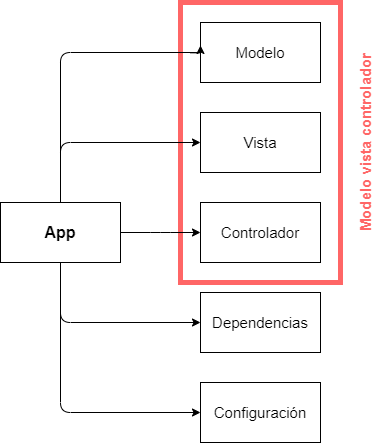
\includegraphics[width=0.6\textwidth]{imagenes/Estructura_carpetas.png}
\caption{Estructura de carpetas de la aplicación}
\label{fig:estructuraCarpetas}
\end{figure}

\subsection{Diagrama de clases}
Para facilitar la comprensión y que los diagramas se puedan interpretar de manera más sencilla, el diagrama de clases se va a dividir en cuatro partes. 
\begin{enumerate}
    \item Análisis: Esta parte se corresponde con el análisis de los mensajes. Estaría dentro del controlador del index y es la parte encargada de extraer los patrones.
    \item Controladores.
    \item Modelos.
    \item Vistas.
\end{enumerate}
\subsubsection{Análisis}
La parte del análisis está compuesta por tres partes (Ver figura \ref{fig:DC_anslisis}):
\begin{enumerate}
    \item Analyzer: Esta clase es la encargada de leer el mensaje en función del formato. 
    \item PatternSearcher: Es la clase encargada de buscar y extraer los patrones mediante las expresiones regulares que están almacenadas en la constante \textit{PATTERNS}. También valida que en el caso de los dominios (O los enlaces o las direcciones de correo) tentan un TDL correcto. 
    \item PatternContainer: En esta clase se almacenarán todos los patrones encargados. Evitará que haya repetidos, añadirá las características y las relaciones necesarias y se encargará de almacenar los datos en la base de datos mendiante el método \textit{save()} 
\end{enumerate}

\begin{figure}[htb]
    \centering
    %\includegraphics[width=0.5\textwidth]{spiral}
    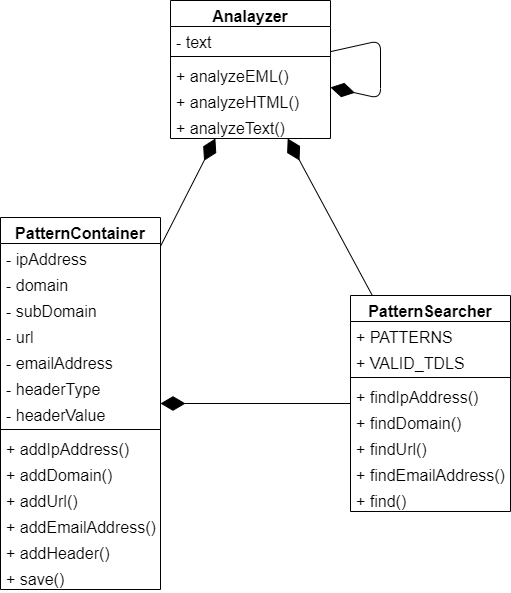
\includegraphics[width=0.6\textwidth]{imagenes/DiagramasClases/Analizador.png}
\caption{Estructura de carpetas de la aplicación}
\label{fig:DC_anslisis}
\end{figure}

\subsubsection{Controladores}
Los controladores permiten al usuario navegar por la web, en el controlador index es donde se permite al usuario enviar a analizar los correos, los demás son de consulta (correos, direcciones IP, dominios, enlaces y direcciones de correo).

Un ejemplo de controlador sería el código \ref{Codigo:controlador}

\begin{lstlisting}[
    language=PHP,
    breaklines, 
    caption={Ejemplo de controlador}, 
    label={Codigo:controlador}, 
    captionpos=b]
    class Domain extends Controller
    {	
        function __construct($request){
            parent::__construct('Domain.html', $request);
        }
        public function render(){

            $value = $this->request->getNextElement();
            if($value){
                $info = DataAccessObjectFactory::getDataAccessObject("DomainDAO_SQL_PDO")->getInfo($value);
                $this->addArgument("info", $info);
            }
            return parent::renderDirectly();
        }
    }
\end{lstlisting}

Todos los controladores heredan de una clase abstracta llamada Controller (Ver figura \ref{fig:DC_controladores}), en ella se almacenan todos los métodos genéricos, como la llamada a la librería de Twig o el nombre de la vista. También se crea un objeto Request en el que almacena información sobre la dirección en la que el usuario a clicado, esto permite al controlador saber qué vista debe generar y a qué modelo llamar. 

\paragraph{Clase Controller}
De esta clase destacan los siguientes métodos: 
\begin{itemize}
    \item notFound: se utiiza si se intenta acceder a una URL que el controlados no conoce. 
    \item addArgument: permite a las clases que heredan de ella añadir argumentos que se pasarán a la vista.
    \item render: es el método que genera la vista y la envía una vez que tiene todos los argumentos necesarios para generarla. 
\end{itemize}

\paragraph{Clase Request}
De esta clase destacan los siguientes métodos: 
\begin{itemize}
    \item getMethod: indica si el método con el que se hace la petición a Apache es get o Post.
    \item getNextElement: devuelve la siguiente parte del path si este está separado mediante ``\verb!/!''.
\end{itemize}

\begin{figure}[htb]
    \centering
    %\includegraphics[width=0.5\textwidth]{spiral}
    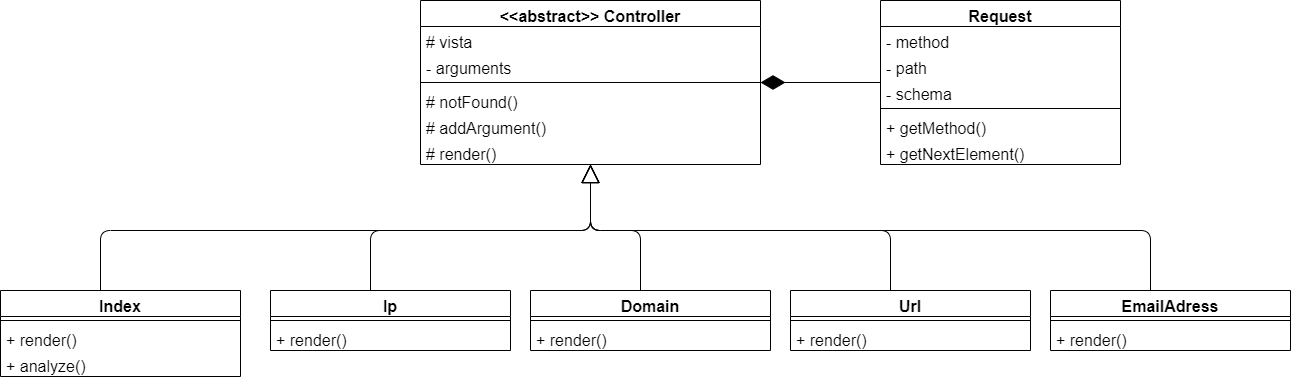
\includegraphics[width=0.8\textwidth]{imagenes/DiagramasClases/Controladores.png}
\caption{Diagrama de clases de los controladores}
\label{fig:DC_controladores}
\end{figure}

\subsubsection{Modelos}
Los modelos son los únicos encargados de interactuar con la base de datos, para hacer esto se ha hecho uso de la clase PDO de PHP, ya que aporta seguridad respecto a mysqli \cite{why_pdo_vs_msqli} y permite una migración sencilla a otro tipo de gestor de base de datos, como ya se ha mencionado (Ver apartado \ref{php_bases_de_datos}).

Para esto se ha utilizado la figura del Objeto de acceso a datos (DAO del inglés Data Access Object). Para evitar duplicar código, se ha creado una clase abstracta genérica llamada DataAccessObjectPDO de la cual extenderán las demás (Ver figura \ref{fig:DC_modelos}).

Esta clase está compuesta por un objeto de la clase DataBasePDO, en él se leerá un archivo de configuración con los parámetros de conexión a la base de datos. 
El separar estos dos objetos se hace para que puedan coexistir dos bases de datos al mismo tiempo.

\paragraph{Clase DataAccessObjectPDO}

De esta clase destacan los siguientes métodos: 
\begin{itemize}
    \item getConnection: Se utiliza para realizar la conexión con la base de datos. 
    \item getConnectionReadOnly: Es similar al método anterior, pero no se podrán leer datos.
    \item getItems: Es un método genérico para poder obtener todos los datos de la tabla del modelo actual.
    \item pagination: permite obtener una fracción de los datos de la tabla del modelo actual.
    \item prepare: genera una consulta preparada. 
    \item hash: se utiliza para generar el hash dado el valor. 
    \item findOrInsertFromArrayValues: permite obtener información a partir de un array de datos y en caso de no encontrarse, se insertan los elementos. 
    \item insertOrUpdateFromArrayValues: Se inserta un array de datos y en caso de existir ya el elemento, lo actualiza. 
\end{itemize}

Las clases que hereden de esta, tendrán que implementar dos métodos, \textit{getInfo()}, que se usa para obtener la información necesaria para la vista e \textit{insert()} que permite insertar objetos desde los métodos \textit{findOrInsertFromArrayValues()} o \textit{insertOrUpdateFromArrayValues()}. 


\begin{figure}[htb]
    \centering
    %\includegraphics[width=0.5\textwidth]{spiral}
    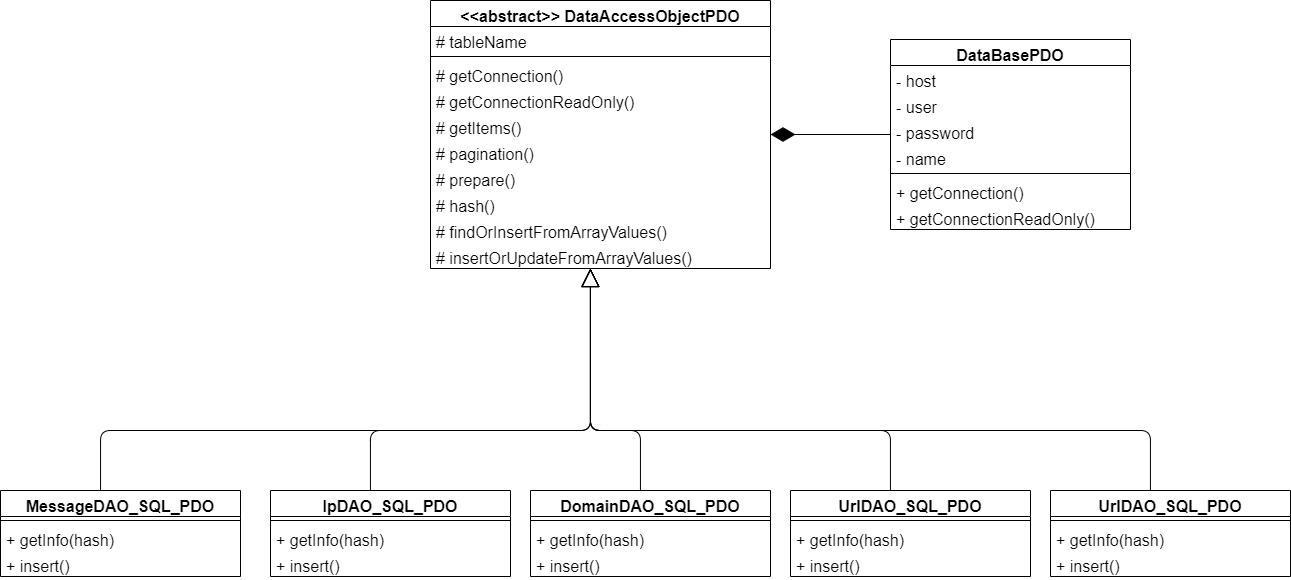
\includegraphics[width=0.8\textwidth]{imagenes/DiagramasClases/Modelos.png}
\caption{Diagrama de clases de los modelos}
\label{fig:DC_modelos}
\end{figure}

\subsubsection{Vistas}
Al ser una aplicación web, las vistas están hechas con HTML, CSS y JavaScript. En esta parte se ha utilizado Twig como gestor de plantillas y Bootstrap como librería para el diseño de la web. 

\paragraph{Twig}
Twig es un gestor de plantillas desarrollado por Symfony \cite{Twig} para PHP. Esto facilita la reutilización de código y el paso de información del modelo a la vista.

Gracias a la propiedad de herencia de Twig \cite{twig_extends}, se ha creado una plantilla base de la que heredarán las demás, de esta manera toda la información que es común se mantiene a lo largo de todas las vistas sin tener que repetir código, como por ejemplo la parte del header o del footer (ver figura \ref{fig:DC_vistas}). También se importará Bootstrap. 

\paragraph{Bootstrap}
Bootstrap es una librería desarrollada por Twitter con una gran cantidad de opciones y facilidades para el diseño web \cite{Bootstrap}. 
Se ha utilizado sobre todo para hacer la web adaptable a dispositivos móviles.

\begin{figure}[htb]
    \centering
    %\includegraphics[width=0.5\textwidth]{spiral}
    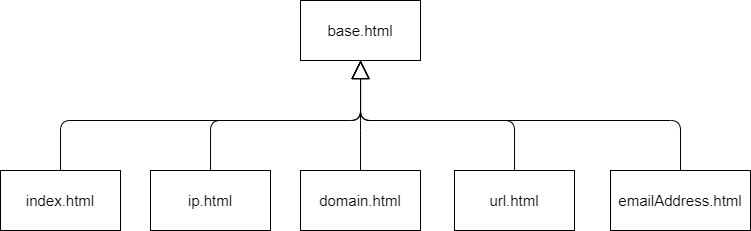
\includegraphics[width=0.8\textwidth]{imagenes/DiagramasClases/Vistas.png}
\caption{Diagrama de clases de las vistas}
\label{fig:DC_vistas}
\end{figure}

\subsection{Diagrama de flujo}
\subsubsection{Modelo Modelo-Vista-Controlador}\label{diagrama_MVC}
El modelo Modelo-Vista-Controlador se puede explicar mediante la secuencia sigueinte (Ver figura \ref{fig:MVC}): 
\begin{enumerate}
    \item El cliente realiza una acción que es capturada por el controlador. 
    \item El controlador elige un modelo, que se encarga de acceder a la base de datos y obtener la información necesaria. 
    \item El modelo le envía la información obtenida al controlador. 
    \item El controlador elige la vista adecuada y le pasa la información recibida del modelo. 
    \item La vista interpreta la información, en base a ella genera la vista final y se la envía al controlador. 
    \item El controlador le envía la vista ya formada al cliente. 
\end{enumerate}

\begin{figure}[htb]
    \centering
    %\includegraphics[width=0.5\textwidth]{spiral}
    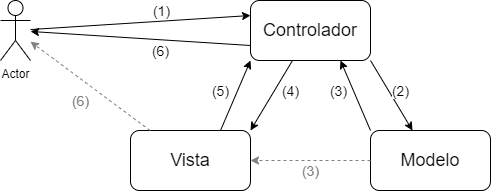
\includegraphics[width=0.8\textwidth]{imagenes/DiagramasFlujo/Modelo_Vista_Controlador.png}
\caption{Diagrama de flujo del modelo Modelo-Vista-Controlador}
\label{fig:MVC}
\end{figure}

\subsubsection{Diagrama de flujo al llegar un nuevo mensaje}
Al llegar un nuevo mensaje se siguen los siguientes pasos: 
\begin{enumerate}
    \item Se consulta si el correo ya ha sido analizado, en caso de haber sido analizado, se devuelve la información que haya en la base de datos.
    \item En caso de no haber sido analizado, en función del formato del mensaje se siguen los siguientes pasos.
        \begin{enumerate}
            \item EML: Si el formato es EML y tiene algún mensaje en el interior, se enviarán al punto 1 todos los mensajes que tengan.
            A continuación se analizarán las cabeceras, extrayendo por un lado el tipo y por otro el valor. 
            \begin{verbatim}
<Tipo de cabecera>:<valor>
            \end{verbatim}
            Dentro de valor se intentarán extraer todos los posibles patrones como si se tratase de un texto. 
            \item HTML: Si el mensaje está en formato HTML se observarán las etiquetas <a>, en concreto el valor del atributo “href” y del texto mostrado al usuario. 
            \item Texto plano: Si el formato es texto plano, simplemente se extraen todos los patrones mediante expresiones regulares y se almacenan.
        \end{enumerate}
\end{enumerate}

Hay que tener en cuenta que un texto en formato EML puede tener contenidos varios textos en varios formatos. Ver figura \ref{fig:nuevoMensaje}

\begin{figure}[htb]
    \centering
    %\includegraphics[width=0.5\textwidth]{spiral}
    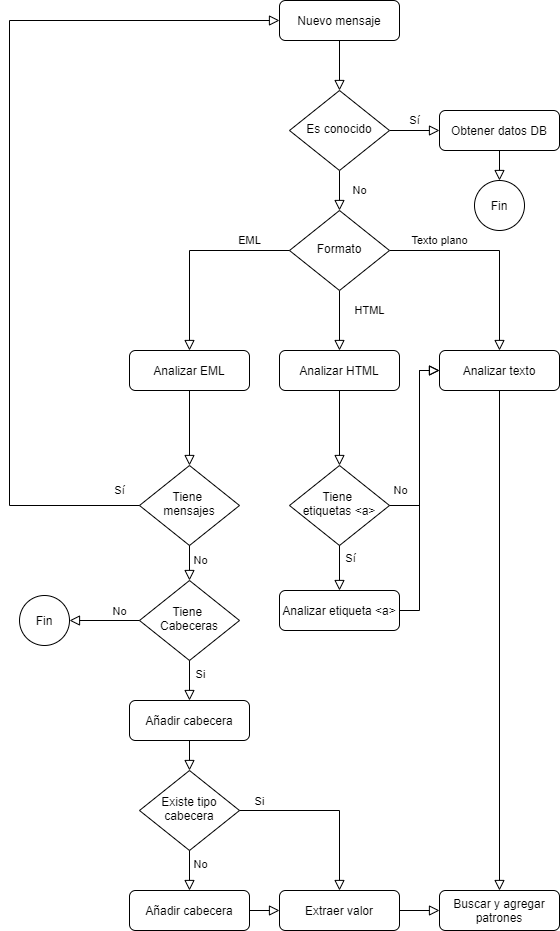
\includegraphics[width=0.8\textwidth]{imagenes/DiagramasFlujo/NuevoMensaje.png}
\caption{Diagrama de flujo cuando llega un nuevo mensaje}
\label{fig:nuevoMensaje}
\end{figure}

\cprotect\subsubsection{Diagrama de flujo para analizar una etiqueta \verb!<a>!}

Para analizar la etiqueta \verb!<a>!, esta debe tener un atributo “href” y texto. Si ambos coinciden, no se hace nada, en caso contrario, se aumenta el score del patrón del atributo “href”. Ver figura \ref{fig:etiquetas_a}.

\begin{figure}[htb]
    \centering
    %\includegraphics[width=0.5\textwidth]{spiral}
    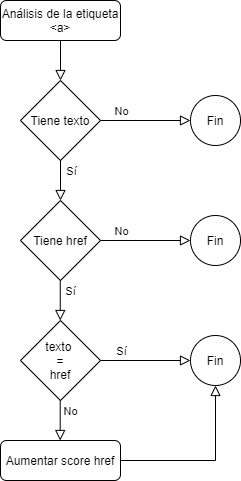
\includegraphics[width=0.4\textwidth]{imagenes/DiagramasFlujo/etiqueta_a.png}
\caption{Diagrama de flujo para analizar las etiquetas 
\texttt{<a>}}
\label{fig:etiquetas_a}
\end{figure}


\subsubsection{Diagrama de flujo para analizar una etiqueta}
En este apartado se irá comprobado si en el texto se encuentran patrones de los que se han obtenido las expresiones regulares en el punto \ref{imp:expresiones_regulares}. En caso de que haya, se comprobará si tiene características maliciosas como las mencionadas en el punto \ref{patrones_maliciosos}, en caso de tener alguna de ellas, se aumentará su score y se almacenará.  Ver figura \ref{fig:patrones}.

\begin{figure}[htb]
    \centering
    %\includegraphics[width=0.5\textwidth]{spiral}
    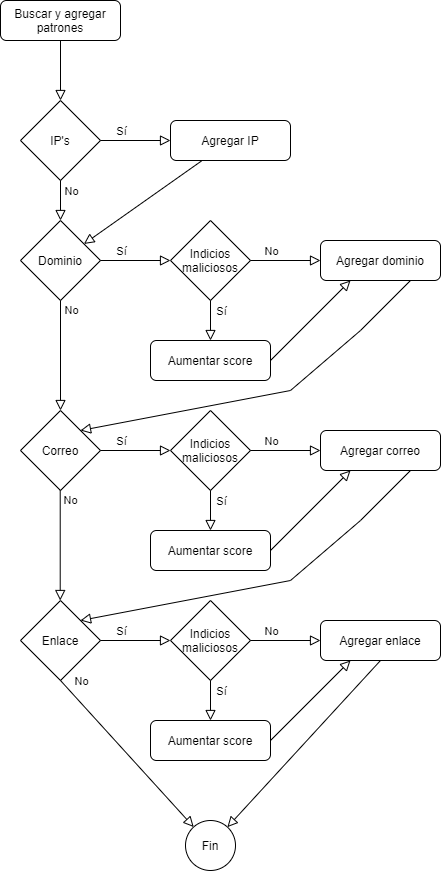
\includegraphics[width=0.6\textwidth]{imagenes/DiagramasFlujo/Buscar_agregar_patrones.png}
\caption{Diagrama de flujo para buscar y almacenar patrones}
\label{fig:patrones}
\end{figure}

\section{Capturas de pantallas}

\subsection{Index}
\begin{figure}[H]
    \centering
    %\includegraphics[width=0.5\textwidth]{spiral}
    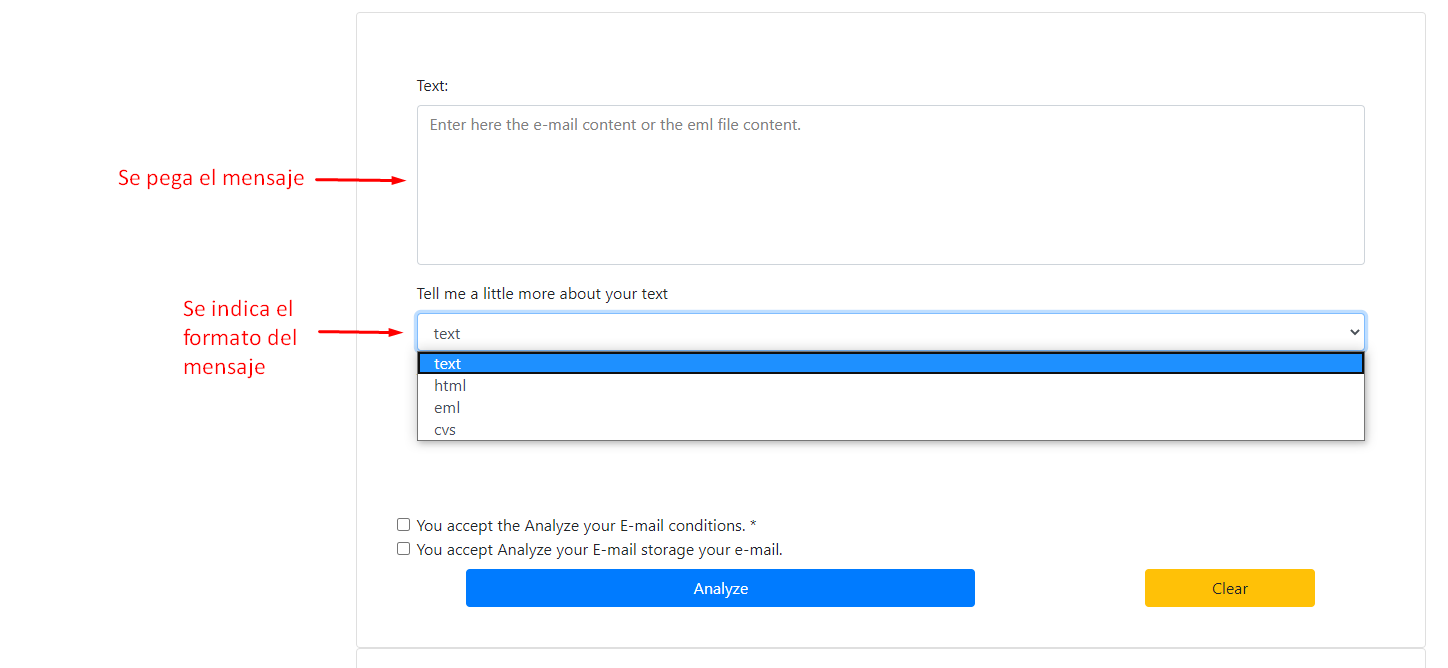
\includegraphics[width=0.9\textwidth]{imagenes/capturasAplicacion/Analizar_mensaje.png}
\caption{Index de la aplicación}
\label{fig:index}
\end{figure}

\subsection{Mensaje}
\begin{figure}[H]
    \centering
    %\includegraphics[width=0.5\textwidth]{spiral}
    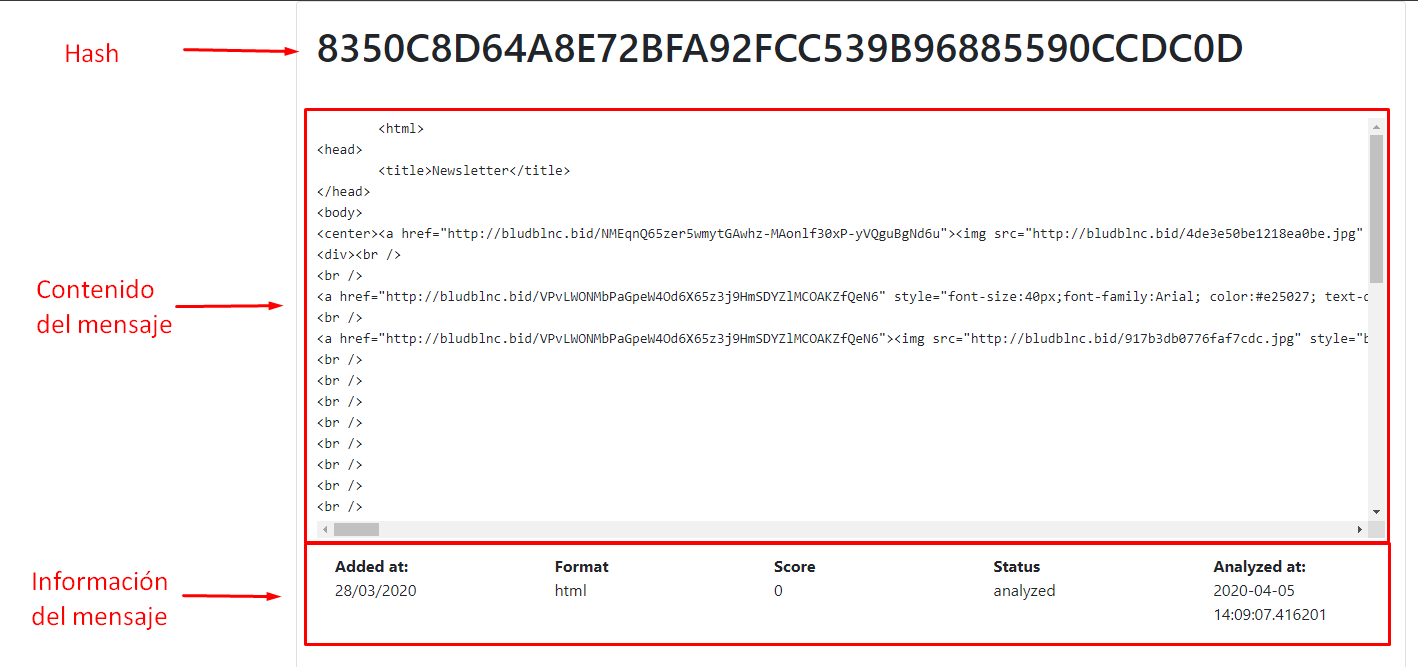
\includegraphics[width=0.9\textwidth]{imagenes/capturasAplicacion/Mensaje_info.png}
\caption{Vista de un mensaje: Información básica}
\end{figure}

\begin{figure}[H]
    \centering
    %\includegraphics[width=0.5\textwidth]{spiral}
    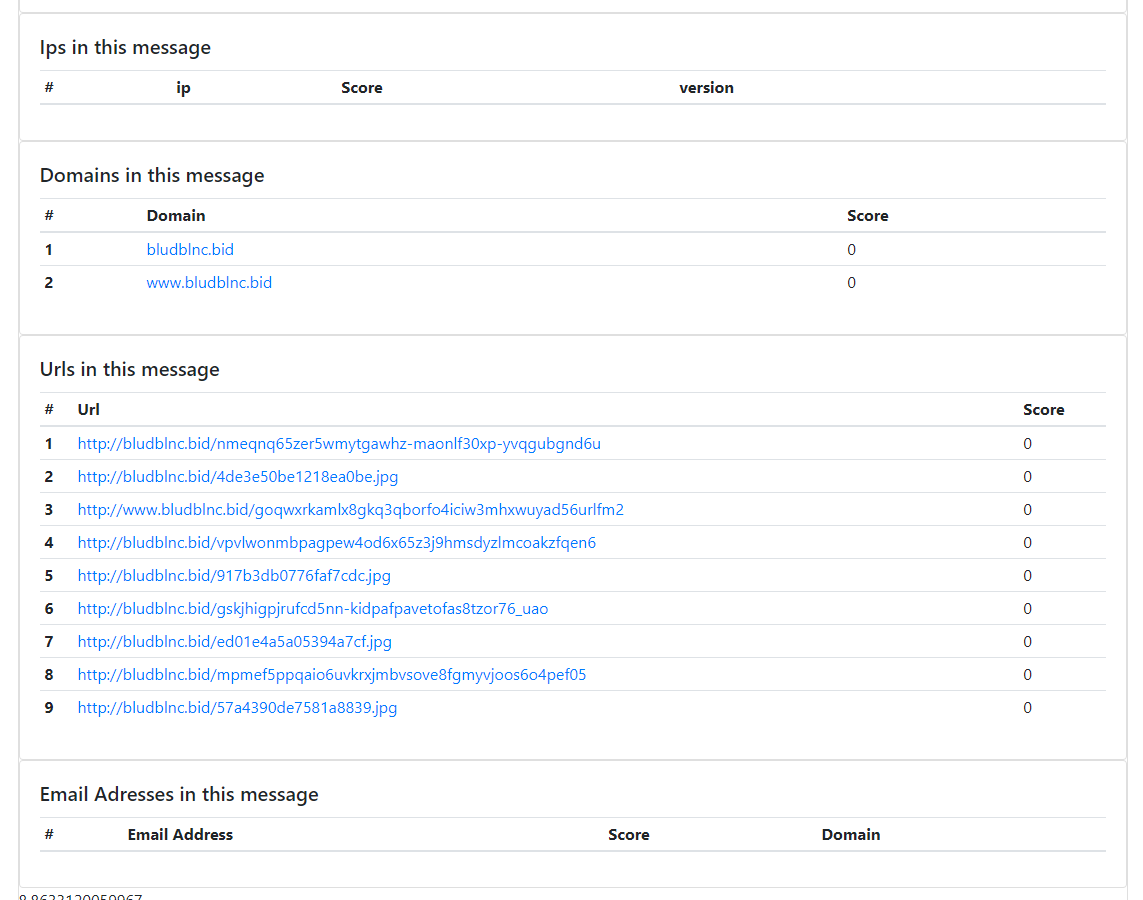
\includegraphics[width=0.9\textwidth]{imagenes/capturasAplicacion/Mensaje_patrones.png}
\caption{Vista de un mensaje: Patrones}
\end{figure}